
\section{Abstract Framework}\label{sec:framework}

% In the current state of the field of structural health monitoring, regardless of the method employed, evaluations rely on some form of \emph{model} that is created to predict some form of \emph{metric} describing structural behavior for a given excitation. The structure experiences service-level conditions for long periods of time, during which structural behavior remains within an ostensibly predictable range. This concept has been shown during the first trial operational period of the \BRACE{} health monitoring platform. Throughout, the bridge inventory has been subject to low levels of excitation. On the health monitoring platform, physics-based methods are primarily used to report intensity measures, and data-driven methods to report deviations from the normal condition. For both types of methods, there is great use in investigating structural behavior as a \emph{linear time invariant} (LTI) system during the normal condition. This allows the physics-based modeler to tailor modeling assumptions for different cases of excitation, and the data-driven modeler to characterize the normal linear system behavior. Several promising formulations for LTI systems have been established for both physics-based and data-driven models, and the \BRACE{} platform allows for their long-term proof-of-concept and validation.

\begin{figure}[h]
    \centering
    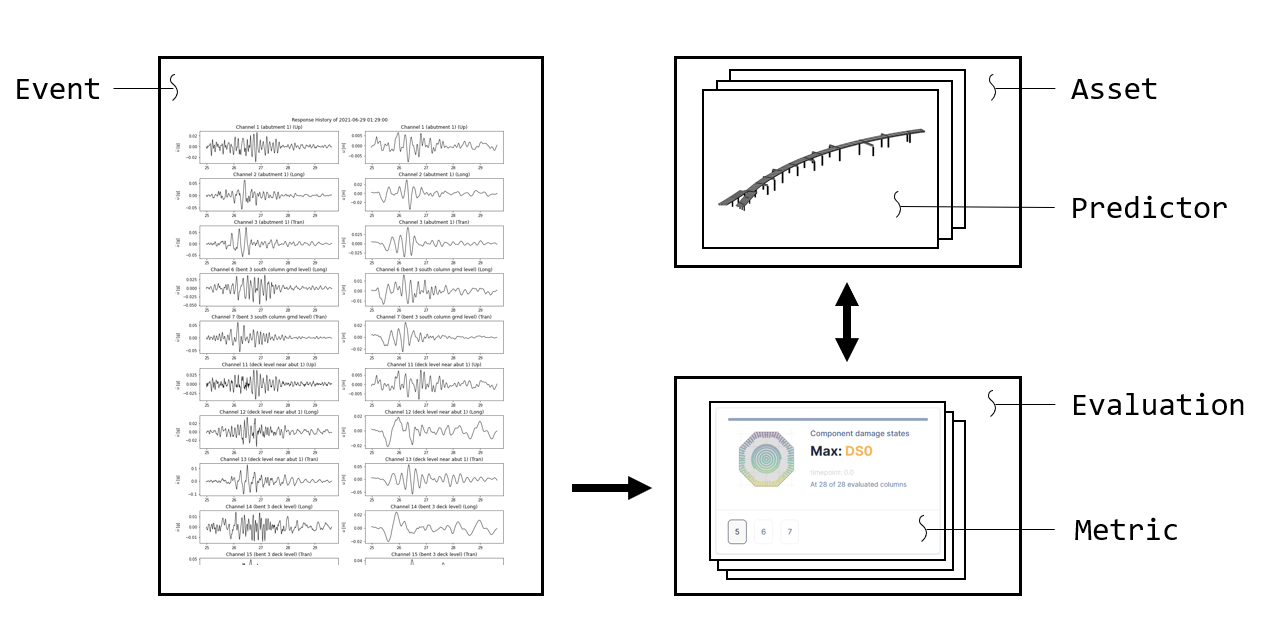
\includegraphics[width=0.9\textwidth]{Body/Irie/Figures/abstractions.png}
    \caption{The \gls{asset}, \gls{predictor}, \gls{event}, \gls{evaluation}, and \gls{metric} represent the central abstractions of the \BRACE{} platform for bridge health monitoring.}
    \label{fig:abstractions}
\end{figure}

The central objectives of structural health monitoring are represented by five key abstractions (\cref{fig:abstractions}): \glspl{asset}, \glspl{event}, \glspl{evaluation}, \glspl{predictor}, and \glspl{metric}.
These abstractions each embody an essential component of a complete structural health monitoring framework.
An \gls{asset} is a unique physical object for which there is interest in its structural health. 
The term \gls{metric} is used to refer to those final quantities that are presented before a decision maker and serve as indicators of structural health or damage. 
These metrics are analogous to indicators like body temperature and heart rate that a medical specialist uses to diagnose a sick patient. They are computed, in real time or near real time, following \glspl{event}, e.g., a major earthquake or a man-made accident, due to pre-defined triggering mechanisms and their associated thresholds. Health metrics are generated by \glspl{predictor}, which either simulate the structural response or identify the structural properties.
In order to conduct a meaningful structural health assessment, the assessor must have a sound understanding of how each metric is composed and interpreted.

%
%
%
\subsection{Assets}\label{sec:assets}
The \gls{asset} abstraction represents the primary subject of structural health monitoring. For example, the Painter St. Overcrossing in \cref{fig:continuous-flare} (a) is an \gls{asset} identified with station number \texttt{CE89324} of the California Strong Motion Instrumentation Program (CSMIP) and structure number \texttt{04 0236} in the Federal Highway Administration’s National Bridge Inventory.
Naturally, an inventory of \glspl{asset} will consist of a wide variety of structural designs, each with distinct vulnerabilities and strengths. 
It is essential that the representation of an \gls{asset} is able to account for these contextual details.
For example, several older bridges in the Caltrans inventory, including the Painter St. overcrossing, are designed with continuous flared columns like that shown in \cref{fig:continuous-flare} (a).  
Structures with this design are particularly vulnerable to certain failure modes as shown in \cref{fig:continuous-flare} (b) \citep{sanchez1997seismic,soleimani2017seismic,caltrans2009memo-6-1}.
% An asset must be represented by a well-defined schema.

\begin{figure}[h!]
    \centering
    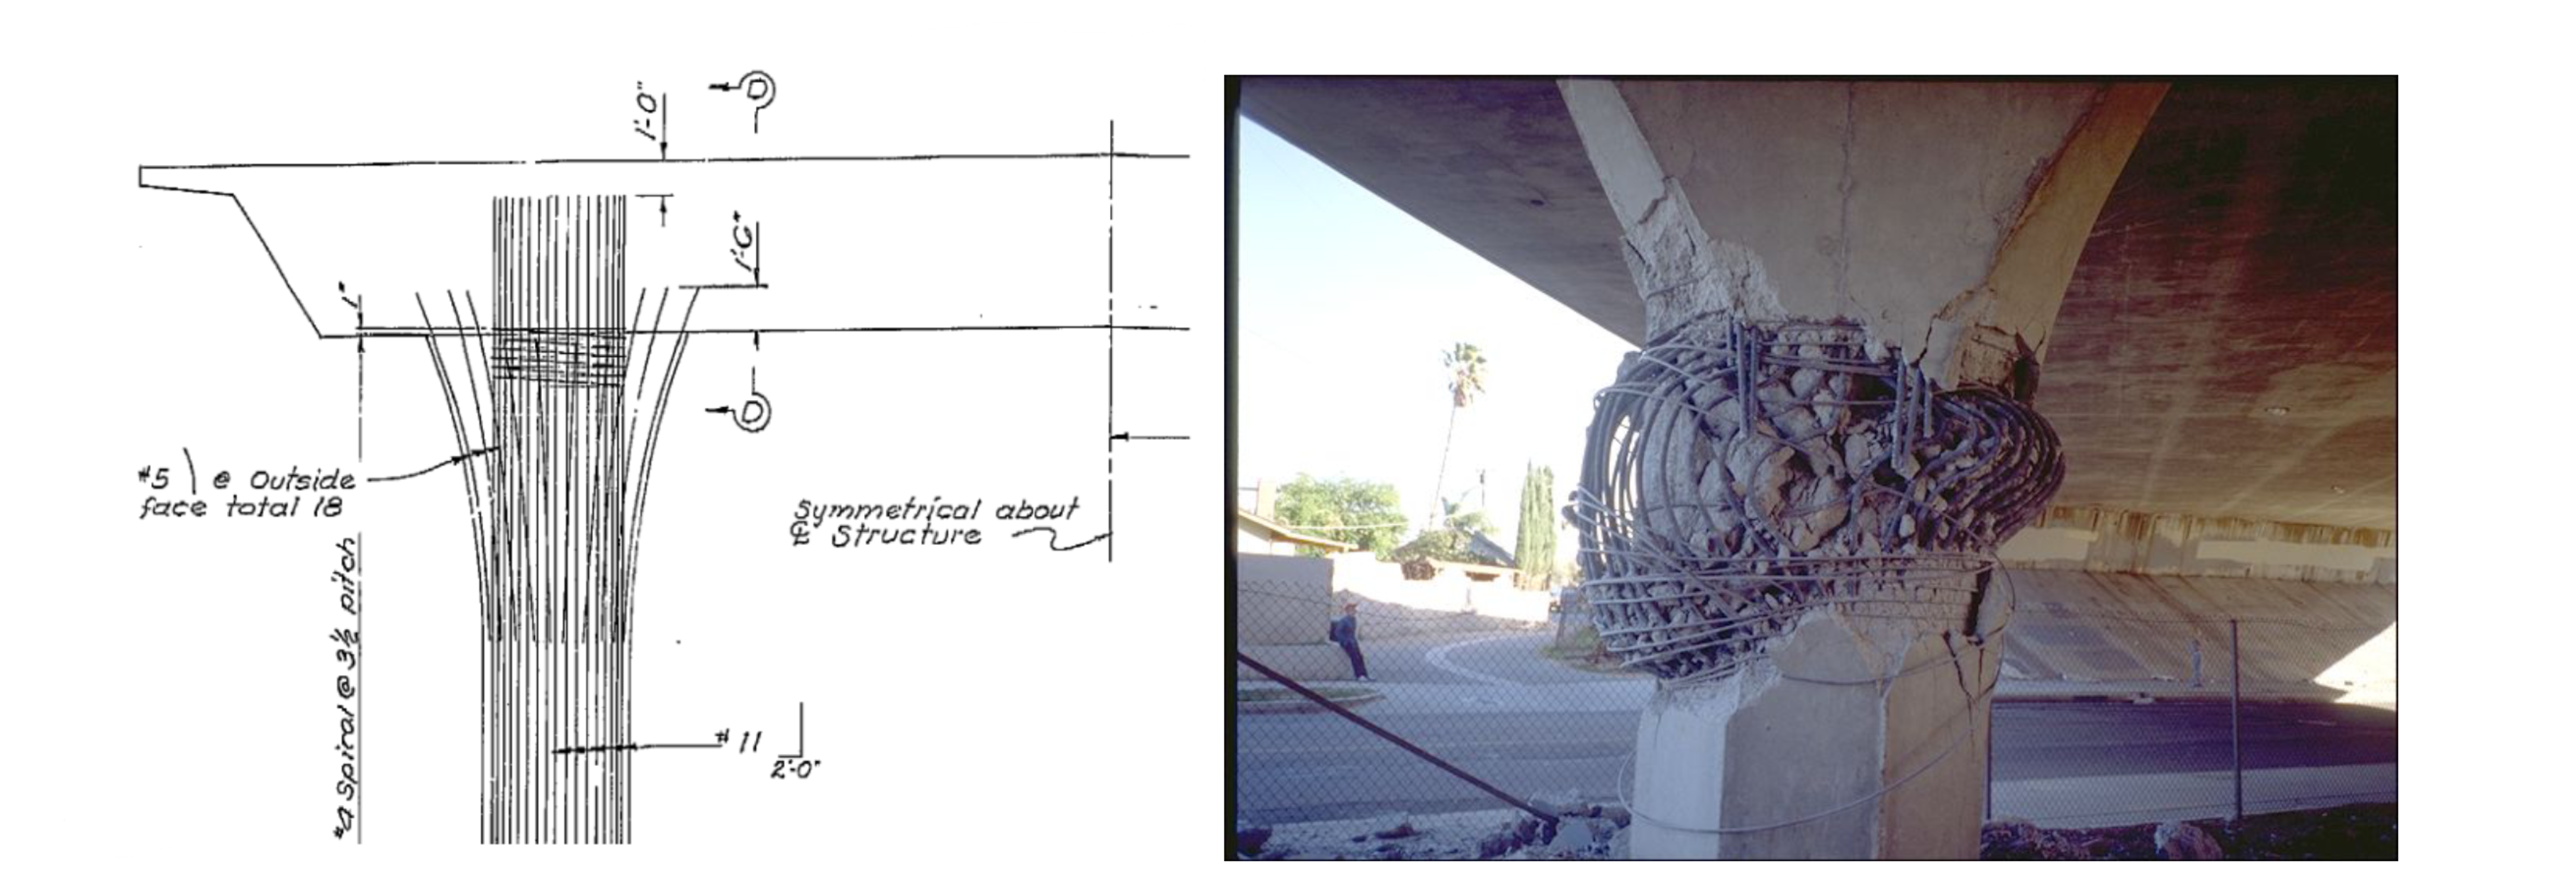
\includegraphics[width=\textwidth]{Body/Irie/Figures/obsolete-flare.png}
    % 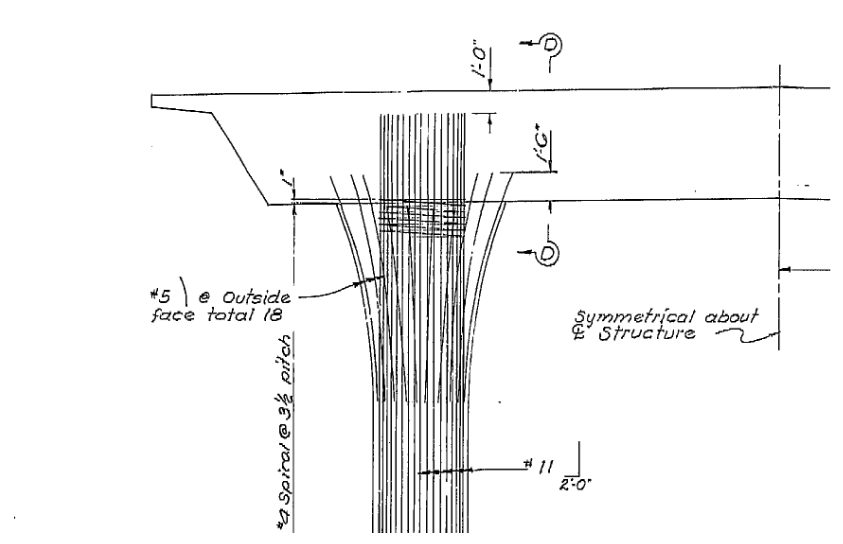
\includegraphics[width=0.5\textwidth]{Body/Irie/Figures/Screenshot 2024-02-02 193305.png}
    % 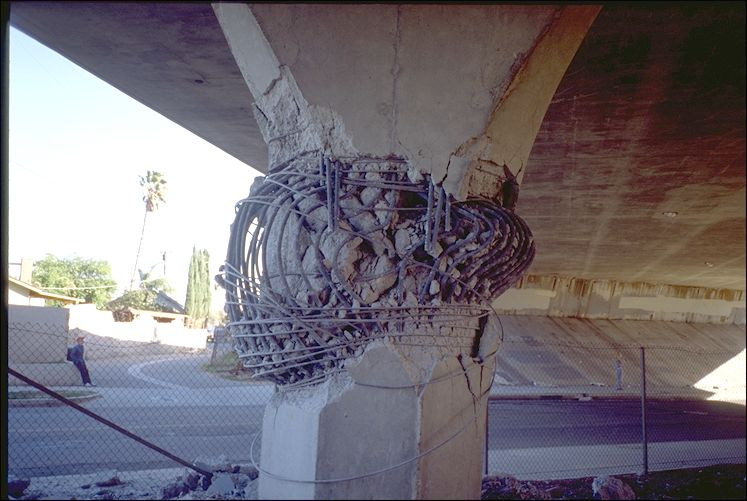
\includegraphics[width=0.45\textwidth]{Body/Irie/Figures/IMG0036.jpg}
    \caption{Example of an important feature included in the representation of an \gls{asset}. Left: Obsolete continuous flare detail from the Painter St. overcrossing. Right: Column failure of the Mission Gothic Bridge following the 1994 Northridge earthquake (Photo courtesy of PEER NISEE, \cite{aschheim1994mission}).}
    \label{fig:continuous-flare}
\end{figure}

\subsection{Predictors}
\begin{figure}[h!]
    \centering
    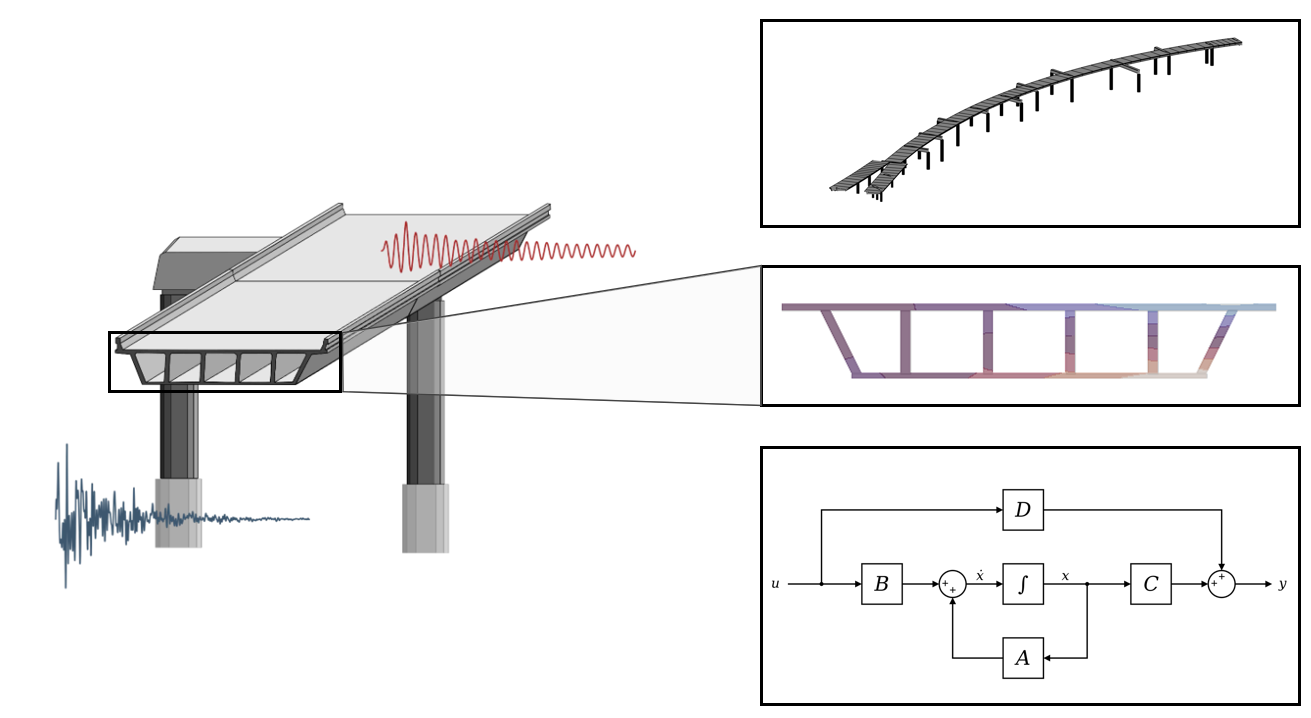
\includegraphics[width=0.95\textwidth]{Body/Irie/Figures/predictors.png}
    % \includegraphics[width=0.45\textwidth]{Body/Irie/Figures/painter-transverse2.pdf}
    % 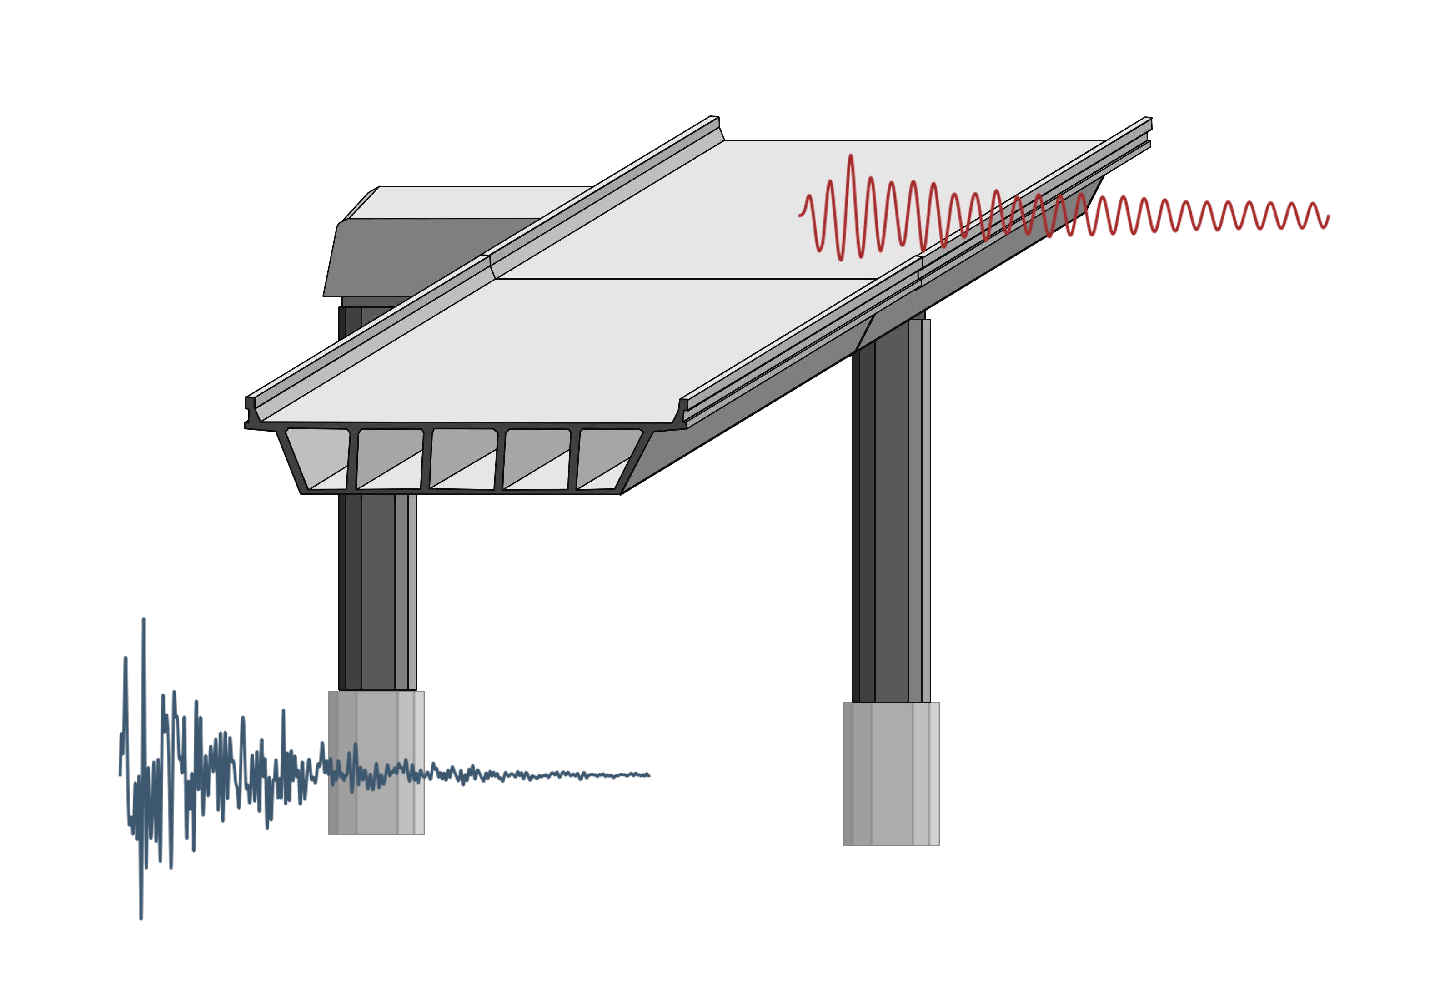
\includegraphics[width=0.45\textwidth]{Body/Irie/Figures/sysid_sensors.pdf}
    \caption{A depiction of an Asset (left) alongside three associated Predictors (right). The depicted predictors are (from top to bottom) a nonlinear finite element model for the dynamic equilibrium problem, a linear finite element model for the plane warping problem, and a system identification model for a state-space realization of the inverse dynamic equilibrium problem.}
    \label{fig:overview-predictors}
\end{figure}

The \gls{predictor} abstraction represents procedures that implement a mathematical model of a physical system.
This abstraction encapsulates the complexity of various modeling techniques and offers a unified interface for predicting system behavior. 
This generally includes any analysis procedure
that an engineer can configure beforehand to be run when an \gls{event} is triggered. 
This covers both methods based on conventional structural analysis and methods 
based on data fitting.
% Examples of predictors include system identification methods and finite element models, each with their unique approaches to modeling physical systems.
Because of the rate of active development in the 
 field of structural health monitoring, the development of these procedures is expected to continue growing.
 
It is useful to consider prediction methods as belonging to one of two families: 
\glspl{predictor-t1} and \glspl{predictor-t2}. 
In both cases, the \gls{predictor} is defined through a \emph{Physics-Driven, Data-Informed} 
paradigm, such that 
the state of a structure as it experiences an \gls{event} is assumed to be characterized by its displacement $\displ$ and velocity $\veloc$, which is governed by Newton's laws of motion \cite{arnold1978mathematical}:
\begin{equation}
    \Mass \accel = \extern -  \intern(\displ,\veloc), %\force (\displ, \veloc, \accel) = \mathbf{f}.
    \label{eq:newton-discrete}
\end{equation}
Here $\accel$ is the acceleration associated with the state of the structure, $\intern$ characterizes the internal resisting force produced by the structure in response to its configuration, and $\extern$ is the external loading that is imposed by the \gls{event}. 

\subsubsection{Type I: Forward Methods}

In the context of \eqref{eq:newton-discrete}, \glspl{predictor-t1} answer the problem statement:
\begin{quote}
 % are premised on the idea that 
 If the form of $\intern$ is \emph{assumed} and the loading $\extern$ is \emph{given}, then $\displ$ and $\veloc$ can be approximately \emph{determined}.
\end{quote}
%
\glspl{predictor-t1} are commonly realized as approximate models for boundary value problems on infinite-dimensional (Hilbert) vector spaces by employing a \emph{finite element} discretization to furnish $\Mass$ and $\intern$ and an approximation to $\extern$ is constructed from input sensor data. 
Highly nonlinear geometric phenomena like buckling and collapse are efficiently represented by generalizing to the setting of infinite-dimensional manifolds \cite{perez2024nonlinear}.
Finite elements models as \glspl{predictor} have recently been considered in the context of digital twins by \cite{torzoni2024digital,ghahari2022bridge,chern2024brace2}. 
These techniques are particularly
attractive because they are readily
accessible to the large workforce of civil engineers that routinely develops models of
this type for problems in design and rehabilitation.
%
However, conventional approaches to constructing such models can be 
extremely costly to produce at scale, as they require a qualified engineer to carefully characterize the properties of each structural component.

Alternatively, \glspl{predictor-t1} may be realized through artificial intelligence models that have been trained to approximate the response of a finite element model (see, e.g.,  \cite{pang2024deep}). Although the field is still in its infancy, this approach may be particularly important in cases where transferable models can be achieved. %\cite{mosalam2024artificial}.

% It is important to note that developing a finite element model for structural health monitoring is fundamentally distinct from the more typical practice of modeling for design or rehabilitation. Many common guidelines and best practices which have been developed for these latter purposes would not generally be well suited for structural health monitoring.


\subsubsection{Type II: Inverse Methods}
In the context of \eqref{eq:newton-discrete}, \glspl{predictor-t2} answer the problem statement:
\begin{quote}
 %are premised on the idea that 
 If general constraints on $\Mass$ and $\intern$ are \emph{assumed} and $\extern$ and $\accel$ are \emph{given}, then the function $\intern$ can be approximately \emph{determined}.
\end{quote}
%
\glspl{predictor-t2} are particularly amenable to data-driven methods.
%
Data-driven methods take advantage of measured response quantities to reduce the number of modeling parameters when an analyst is faced with the challenge of defining them in \glspl{predictor-t1}.
This reduction can be quite significant, and with adequate data sources, can be accurately configured in just hours, as opposed to the weeks
that an engineer may typically require to assemble a traditional structural analysis model of a bridge system.

For example, a \glspl{predictor-t2} may be realized by prescribing the domain and range of $\intern$ and then using \emph{system identification} methods to fit $\intern$ to directly observed loading and acceleration data \citep{arici2003system,chern2024crosssectional}.
% An important class of data-driven methods include those for \emph{system identification}. 
Methods of system identification use recorded response histories to characterize the system dynamics of the structure at hand. These dynamics are expressed in terms of either an input-output relationship in the frequency domain, called a transfer function, or a state space representation in the time domain, which is a set of first-order differential equations. 
Generally, the parameters of the dynamic equilibrium equations are used as identifying characteristics of the structure. 
Health monitoring then entails tracking the data-fitted identity of a structure over time.

\subsection{Metrics}
\begin{figure}[H]
    \centering
    \resizebox{0.9\linewidth}{!}{% generated by Plantuml 1.2025.4       
\definecolor{plantucolor0000}{RGB}{255,255,255}
\definecolor{plantucolor0001}{RGB}{0,0,0}
\definecolor{plantucolor0002}{RGB}{194,194,194}
\definecolor{plantucolor0003}{RGB}{24,24,24}
\definecolor{plantucolor0004}{RGB}{84,84,84}
\definecolor{plantucolor0005}{RGB}{166,166,166}
\begin{tikzpicture}[yscale=-1
,pstyle0/.style={color=black,fill=white,line width=0.5pt}
,pstyle1/.style={color=plantucolor0003,fill=plantucolor0002,line width=1.0pt}
,pstyle2/.style={color=black,line width=0.5pt}
,pstyle3/.style={color=plantucolor0004,line width=1.0pt}
,pstyle4/.style={color=plantucolor0004,fill=plantucolor0005,line width=1.0pt}
,pstyle5/.style={color=black,line width=1.0pt}
]
\draw[pstyle0] (219.3pt,12pt) arc (180:270:5pt) -- (224.3pt,7pt) -- (325.7pt,7pt) arc (270:360:5pt) -- (330.7pt,12pt) -- (330.7pt,100pt) arc (0:90:5pt) -- (325.7pt,105pt) -- (224.3pt,105pt) arc (90:180:5pt) -- (219.3pt,100pt) -- cycle;
\draw[pstyle1] (257.142pt,23pt) ellipse (11pt and 11pt);
\node at (257.142pt,23pt)[]{\textbf{\Large C}};
\node at (276.218pt,18pt)[below right,color=black,inner sep=0]{Metric};
\draw[pstyle2] (220.3pt,39pt) -- (329.7pt,39pt);
\draw[pstyle3] (230.3pt,50pt) ellipse (3pt and 3pt);
\node at (239.3pt,43.5pt)[below right,color=black,inner sep=0]{tag : String};
\draw[pstyle3] (230.3pt,61pt) ellipse (3pt and 3pt);
\node at (239.3pt,54.5pt)[below right,color=black,inner sep=0]{payload : Any};
\draw[pstyle4] (230.3pt,72pt) ellipse (3pt and 3pt);
\node at (239.3pt,65.5pt)[below right,color=black,inner sep=0]{verdict() : Enum};
\draw[pstyle5] (220.3pt,77pt) -- (329.7pt,77pt);
\draw[pstyle4] (230.3pt,88pt) ellipse (3pt and 3pt);
\node at (239.3pt,81.5pt)[below right,color=black,inner sep=0]{summary() : String};
\draw[pstyle4] (230.3pt,99pt) ellipse (3pt and 3pt);
\node at (239.3pt,92.5pt)[below right,color=black,inner sep=0]{details() : String};
\draw[pstyle0] (7pt,170pt) arc (180:270:5pt) -- (12pt,165pt) -- (112pt,165pt) arc (270:360:5pt) -- (117pt,170pt) -- (117pt,208pt) arc (0:90:5pt) -- (112pt,213pt) -- (12pt,213pt) arc (90:180:5pt) -- (7pt,208pt) -- cycle;
\draw[pstyle1] (22pt,181pt) ellipse (11pt and 11pt);
\node at (22pt,181pt)[]{\textbf{\Large C}};
\node at (36pt,176pt)[below right,color=black,inner sep=0]{PeriodShiftMetric};
\draw[pstyle2] (8pt,197pt) -- (116pt,197pt);
\draw[pstyle2] (8pt,205pt) -- (116pt,205pt);
\draw[pstyle0] (152.4pt,170pt) arc (180:270:5pt) -- (157.4pt,165pt) -- (252.61pt,165pt) arc (270:360:5pt) -- (257.61pt,170pt) -- (257.61pt,208pt) arc (0:90:5pt) -- (252.61pt,213pt) -- (157.4pt,213pt) arc (90:180:5pt) -- (152.4pt,208pt) -- cycle;
\draw[pstyle1] (167.4pt,181pt) ellipse (11pt and 11pt);
\node at (167.4pt,181pt)[]{\textbf{\Large C}};
\node at (181.4pt,176pt)[below right,color=black,inner sep=0]{PeakAccelMetric};
\draw[pstyle2] (153.4pt,197pt) -- (256.61pt,197pt);
\draw[pstyle2] (153.4pt,205pt) -- (256.61pt,205pt);
\draw[pstyle0] (293.02pt,170pt) arc (180:270:5pt) -- (298.02pt,165pt) -- (393.98pt,165pt) arc (270:360:5pt) -- (398.98pt,170pt) -- (398.98pt,208pt) arc (0:90:5pt) -- (393.98pt,213pt) -- (298.02pt,213pt) arc (90:180:5pt) -- (293.02pt,208pt) -- cycle;
\draw[pstyle1] (308.02pt,181pt) ellipse (11pt and 11pt);
\node at (308.02pt,181pt)[]{\textbf{\Large C}};
\node at (322.02pt,176pt)[below right,color=black,inner sep=0]{DriftRatioMetric};
\draw[pstyle2] (294.02pt,197pt) -- (397.98pt,197pt);
\draw[pstyle2] (294.02pt,205pt) -- (397.98pt,205pt);
\draw[pstyle0] (433.94pt,170pt) arc (180:270:5pt) -- (438.94pt,165pt) -- (539.07pt,165pt) arc (270:360:5pt) -- (544.07pt,170pt) -- (544.07pt,208pt) arc (0:90:5pt) -- (539.07pt,213pt) -- (438.94pt,213pt) arc (90:180:5pt) -- (433.94pt,208pt) -- cycle;
\draw[pstyle1] (448.94pt,181pt) ellipse (11pt and 11pt);
\node at (448.94pt,181pt)[]{\textbf{\Large C}};
\node at (462.94pt,176pt)[below right,color=black,inner sep=0]{StrainStateMetric};
\draw[pstyle2] (434.94pt,197pt) -- (543.07pt,197pt);
\draw[pstyle2] (434.94pt,205pt) -- (543.07pt,205pt);
\draw[pstyle5] (203.7068pt,100.8483pt) ..controls (166.2368pt,123.8883pt) and (133.23pt,144.19pt) .. (100.14pt,164.54pt);
\draw[pstyle5] (219.04pt,91.42pt) -- (200.564pt,95.7372pt) -- (206.8495pt,105.9593pt) -- (219.04pt,91.42pt) -- cycle;
\draw[pstyle5] (240.6505pt,121.2876pt) ..controls (229.8305pt,141.5476pt) and (226.23pt,148.28pt) .. (217.44pt,164.71pt);
\draw[pstyle5] (249.13pt,105.41pt) -- (235.3579pt,118.4611pt) -- (245.943pt,124.1141pt) -- (249.13pt,105.41pt) -- cycle;
\draw[pstyle5] (309.8166pt,121.2353pt) ..controls (320.7966pt,141.4953pt) and (324.47pt,148.28pt) .. (333.38pt,164.71pt);
\draw[pstyle5] (301.24pt,105.41pt) -- (304.5415pt,124.0942pt) -- (315.0917pt,118.3765pt) -- (301.24pt,105.41pt) -- cycle;
\draw[pstyle5] (346.3021pt,100.6474pt) ..controls (384.0721pt,123.7674pt) and (417.58pt,144.28pt) .. (450.91pt,164.68pt);
\draw[pstyle5] (330.95pt,91.25pt) -- (343.1697pt,105.7648pt) -- (349.4346pt,95.5301pt) -- (330.95pt,91.25pt) -- cycle;
\end{tikzpicture}
}
    \caption{Class diagram for the Metric abstraction.}
    \label{fig:metric-class}
\end{figure}
\glspl{metric} represent the various outputs that \glspl{predictor} might produce. They provide a common language for interpreting and comparing the results of different \glspl{predictor}. For instance, both a system identification method and a finite element model can be used to fit modal properties to a given input and output signal. 
Despite these being fundamentally different \glspl{predictor}, the \gls{metric} abstraction allows the modal properties they produce to be presented in a common manner or compared.

The Metric is thus realized as an immutable value object that binds three elements: a tag identifying the physical quantity, a compact payload containing the numerical values, and a verdict that classifies those values against user‑defined thresholds (\cref{fig:metric-class}).  
Because the data, metadata, and judgment travel together, metrics are self‑describing and directly comparable across predictor families.  Whether a frequency shift is inferred by an inverse system‑identification routine or computed by a forward finite‑element simulation, it is exposed through the same interface and can participate in the same decision logic.

Metrics are generally used for two important purposes: they may be passed down to decision-makers to inform judgment calls or fed back to \glspl{predictor} for the purpose of model updating or training \citep{katam2023review,avci2021review}. 

\subsubsection{Metrics for Evaluation}
When metrics are passed to decision-makers, they translate the complex mathematical models into understandable and actionable information. This could be in the form of risk assessments, performance indicators, or any other form of measurement that is relevant to the physical system being modeled. 
By providing a consistent interface for these outputs, the \gls{metric} abstraction ensures that the insights generated by different \glspl{predictor} are comparable and comprehensible, regardless of the underlying prediction method \citep{doebling1998summary,salawu1997detection,dilorenzo2023physics,muin2024human}.
%
% The envisioned judgment calls can include closing a particular bridge, prioritizing locations to send early responders to for in-depth inspection, or declaring that no action is needed. 
\iffalse
In the context of bridges 
% Given this broad range of demands, 
it is useful to distinguish the following applications one may expect a metric to target:

\begin{description}[noitemsep]
    \item [Component condition] which can guide local inspection and repair or retrofit,
    \item [Structure condition] which may guide operational decisions such as road closures, and
    \item [Inventory condition] 
       to facilitate analysis of transportation networks and inspection prioritization.
\end{description}

Engineers will be inclined to target component-level response metrics.  
Such metrics leverage familiar concepts like reinforcing bar strain and can be directly related to well-documented experimental phenomena like concrete confinement or cover spalling.
However, these metrics are likely the least predictable. 
They are most sensitive to the material, geometry, and boundary condition variations, and there can be multiple possible damage states for the same static, and particularly dynamic, loading due to the path-dependent and random characteristics affecting the nonlinear behavior, including soil-foundation-structure interaction and damage propagation. % more reasons
The best use for such metrics is compiling the structure-level condition assessments. For example, evaluation of the overall capacity, stiffness, and ductility of a structure, or estimation of the deviation from the linear elastic range of behavior can give information about the serviceability of the structure that can then be used to make decisions regarding operational actions. Inventory level assessments are expected to be the most reliable and useful, but they depend on concepts that are not part of conventional engineering curricula, such as \emph{regional-scale fragility} and \emph{traffic flow dynamics}.
\fi

\subsubsection{Metrics for Updating}
The second role of metrics is their use in model updating or training. In this scenario, the metrics serve as a feedback mechanism. The outputs of the \glspl{predictor} are evaluated against some desired outcome or benchmark, and this evaluation is fed back into the \gls{predictor}. 
This feedback can be used to adjust the parameters of the \gls{predictor}, effectively ‘training’ it to improve its future outputs \citep{torzoni2024digital,ereiz2022review,ghahari2022bridge}.

The \gls{metric} abstraction is instrumental in this context. It provides a common interface for these evaluations, facilitating the interchangeability of different training algorithms. For instance, consider two distinct \glspl{predictor}: one employing a least squares method for system identification, and another utilizing a genetic algorithm for optimizing a finite element model \citep{gomez-cabrera2022review}. 
Despite the fundamental differences in their methodologies, both \glspl{predictor} can leverage the \gls{metric} abstraction to establish a consistent feedback loop.

This consistency is crucial for several reasons. First, it simplifies the implementation of the training process. 
Regardless of the complexity or nature of the training algorithm, the feedback loop remains the same. 
This uniformity reduces the potential for errors and makes the code easier to understand and maintain.
%
Second, it encourages experimentation with different training algorithms. By abstracting away the details of the feedback loop, the \gls{metric} abstraction allows developers to focus on the training algorithms themselves. They can easily swap in different algorithms, compare their performance, and choose the one that best suits their needs. This flexibility is key to driving innovation and improving the accuracy and efficiency of the \gls{predictor}.

% Finally, the \gls{metric} abstraction also plays a vital role in facilitating collaboration and knowledge sharing. By providing a common language for expressing the outputs of different \glspl{predictor}, it allows developers to share and compare their results, learn from each other’s successes and failures, and collectively push the boundaries of what is possible.

\subsection{Events and Evaluations}\label{sec:events}
% \begin{figure}[H]
%     \centering
%     \resizebox{0.25\linewidth}{!}{% generated by Plantuml 1.2025.4       
\definecolor{plantucolor0000}{RGB}{255,255,255}
\definecolor{plantucolor0001}{RGB}{0,0,0}
\definecolor{plantucolor0002}{RGB}{194,194,194}
\definecolor{plantucolor0003}{RGB}{24,24,24}
\begin{tikzpicture}[yscale=-1
,pstyle0/.style={color=black,fill=white,line width=0.5pt}
,pstyle1/.style={color=plantucolor0003,fill=plantucolor0002,line width=1.0pt}
,pstyle2/.style={color=black,line width=0.5pt}
,pstyle3/.style={color=black,line width=1.0pt}
,pstyle4/.style={color=black,fill=black,line width=1.0pt}
]
\draw[pstyle0] (7pt,16pt) arc (180:270:5pt) -- (12pt,11pt) -- (57.71pt,11pt) arc (270:360:5pt) -- (62.71pt,16pt) -- (62.71pt,54pt) arc (0:90:5pt) -- (57.71pt,59pt) -- (12pt,59pt) arc (90:180:5pt) -- (7pt,54pt) -- cycle;
\draw[pstyle1] (22pt,27pt) ellipse (11pt and 11pt);
\node at (22pt,27pt)[]{\textbf{\Large C}};
\node at (36pt,22pt)[below right,color=black,inner sep=0]{Asset};
\draw[pstyle2] (8pt,43pt) -- (61.71pt,43pt);
\draw[pstyle2] (8pt,51pt) -- (61.71pt,51pt);
\draw[pstyle0] (156.15pt,140pt) arc (180:270:5pt) -- (161.15pt,135pt) -- (208.57pt,135pt) arc (270:360:5pt) -- (213.57pt,140pt) -- (213.57pt,178pt) arc (0:90:5pt) -- (208.57pt,183pt) -- (161.15pt,183pt) arc (90:180:5pt) -- (156.15pt,178pt) -- cycle;
\draw[pstyle1] (171.15pt,151pt) ellipse (11pt and 11pt);
\node at (171.15pt,151pt)[]{\textbf{\Large C}};
\node at (185.15pt,146pt)[below right,color=black,inner sep=0]{Event};
\draw[pstyle2] (157.15pt,167pt) -- (212.57pt,167pt);
\draw[pstyle2] (157.15pt,175pt) -- (212.57pt,175pt);
\draw[pstyle0] (48.47pt,140pt) arc (180:270:5pt) -- (53.47pt,135pt) -- (116.23pt,135pt) arc (270:360:5pt) -- (121.23pt,140pt) -- (121.23pt,178pt) arc (0:90:5pt) -- (116.23pt,183pt) -- (53.47pt,183pt) arc (90:180:5pt) -- (48.47pt,178pt) -- cycle;
\draw[pstyle1] (63.47pt,151pt) ellipse (11pt and 11pt);
\node at (63.47pt,151pt)[]{\textbf{\Large C}};
\node at (77.47pt,146pt)[below right,color=black,inner sep=0]{Predictor};
\draw[pstyle2] (49.47pt,167pt) -- (120.23pt,167pt);
\draw[pstyle2] (49.47pt,175pt) -- (120.23pt,175pt);
\draw[pstyle0] (78.54pt,358pt) arc (180:270:5pt) -- (83.54pt,353pt) -- (134.18pt,353pt) arc (270:360:5pt) -- (139.18pt,358pt) -- (139.18pt,396pt) arc (0:90:5pt) -- (134.18pt,401pt) -- (83.54pt,401pt) arc (90:180:5pt) -- (78.54pt,396pt) -- cycle;
\draw[pstyle1] (93.54pt,369pt) ellipse (11pt and 11pt);
\node at (93.54pt,369pt)[]{\textbf{\Large C}};
\node at (107.54pt,364pt)[below right,color=black,inner sep=0]{Metric};
\draw[pstyle2] (79.54pt,385pt) -- (138.18pt,385pt);
\draw[pstyle2] (79.54pt,393pt) -- (138.18pt,393pt);
\draw[pstyle0] (145.31pt,249pt) arc (180:270:5pt) -- (150.31pt,244pt) -- (219.41pt,244pt) arc (270:360:5pt) -- (224.41pt,249pt) -- (224.41pt,287pt) arc (0:90:5pt) -- (219.41pt,292pt) -- (150.31pt,292pt) arc (90:180:5pt) -- (145.31pt,287pt) -- cycle;
\draw[pstyle1] (160.31pt,260pt) ellipse (11pt and 11pt);
\node at (160.31pt,260pt)[]{\textbf{\Large C}};
\node at (174.31pt,255pt)[below right,color=black,inner sep=0]{Evaluation};
\draw[pstyle2] (146.31pt,276pt) -- (223.41pt,276pt);
\draw[pstyle2] (146.31pt,284pt) -- (223.41pt,284pt);
\draw[pstyle0] (139.31pt,12pt) arc (180:270:5pt) -- (144.31pt,7pt) -- (213.41pt,7pt) arc (270:360:5pt) -- (218.41pt,12pt) -- (218.41pt,58pt) arc (0:90:5pt) -- (213.41pt,63pt) -- (144.31pt,63pt) arc (90:180:5pt) -- (139.31pt,58pt) -- cycle;
\draw[pstyle1] (154.31pt,27pt) ellipse (11pt and 11pt);
\node at (154.31pt,27pt)[]{\textbf{\Large C}};
\node at (171.605pt,12pt)[below right,color=black,inner sep=0]{\textit{\guillemotleft{}service\guillemotright{}}};
\node at (168.31pt,22pt)[below right,color=black,inner sep=0]{Evaluation};
\node at (173.875pt,32pt)[below right,color=black,inner sep=0]{Daemon};
\draw[pstyle2] (140.31pt,47pt) -- (217.41pt,47pt);
\draw[pstyle2] (140.31pt,55pt) -- (217.41pt,55pt);
\draw[pstyle3] (41.18pt,59.37pt) ..controls (45.13pt,72.91pt) and (50.63pt,90.16pt) .. (56.86pt,105pt) ..controls (61.04pt,114.98pt) and (66.45pt,125.6pt) .. (71.39pt,134.69pt);
\node at (37.1602pt,66.8961pt)[below right,color=black,inner sep=0]{1};
\node at (62.3003pt,117.1793pt)[below right,color=black,inner sep=0]{*};
\draw[pstyle3] (184.86pt,183.48pt) ..controls (184.86pt,201.32pt) and (184.86pt,219.75pt) .. (184.86pt,237.57pt);
\draw[pstyle4] (184.86pt,243.57pt) -- (188.86pt,234.57pt) -- (184.86pt,238.57pt) -- (180.86pt,234.57pt) -- (184.86pt,243.57pt) -- cycle;
\draw[pstyle3] (87.42pt,183.12pt) ..controls (92.03pt,224.58pt) and (100.9874pt,305.1767pt) .. (105.6074pt,346.7567pt);
\draw[pstyle4] (106.27pt,352.72pt) -- (109.2517pt,343.3333pt) -- (105.7178pt,347.7506pt) -- (101.3006pt,344.2168pt) -- (106.27pt,352.72pt) -- cycle;
\draw[pstyle3] (168.18pt,292.48pt) ..controls (155.5pt,310.32pt) and (141.6368pt,329.86pt) .. (128.9668pt,347.68pt);
\draw[pstyle4] (125.49pt,352.57pt) -- (133.9652pt,347.5529pt) -- (128.3873pt,348.495pt) -- (127.4452pt,342.9172pt) -- (125.49pt,352.57pt) -- cycle;
\draw[pstyle3] (176.07pt,63.23pt) ..controls (175.18pt,75.94pt) and (174.7pt,91.26pt) .. (175.86pt,105pt) ..controls (176.68pt,114.77pt) and (177.2673pt,119.5367pt) .. (178.9373pt,128.7267pt);
\draw[pstyle4] (180.01pt,134.63pt) -- (182.3364pt,125.0599pt) -- (179.116pt,129.7106pt) -- (174.4653pt,126.4902pt) -- (180.01pt,134.63pt) -- cycle;
\node at (176.86pt,94pt)[below right,color=black,inner sep=0]{receives notification};
\draw[pstyle3] (147.62pt,63.48pt) ..controls (138.42pt,72.39pt) and (128.71pt,82.66pt) .. (120.86pt,93pt) ..controls (111.02pt,105.94pt) and (104.8366pt,116.5301pt) .. (98.3666pt,129.3901pt);
\draw[pstyle4] (95.67pt,134.75pt) -- (103.2882pt,128.5079pt) -- (97.9172pt,130.2834pt) -- (96.1417pt,124.9124pt) -- (95.67pt,134.75pt) -- cycle;
\node at (121.86pt,94pt)[below right,color=black,inner sep=0]{dispatches};
\draw[pstyle3] (218.57pt,50.81pt) ..controls (237.07pt,59.95pt) and (257.29pt,73.68pt) .. (267.86pt,93pt) ..controls (296.61pt,145.56pt) and (248.8176pt,205.4524pt) .. (214.9176pt,239.2724pt);
\draw[pstyle4] (210.67pt,243.51pt) -- (219.8666pt,239.9853pt) -- (214.2097pt,239.9786pt) -- (214.2164pt,234.3218pt) -- (210.67pt,243.51pt) -- cycle;
\node at (276.59pt,154pt)[below right,color=black,inner sep=0]{aggregates};
\end{tikzpicture}
}
%     \resizebox{0.25\linewidth}{!}{% generated by Plantuml 1.2025.4       
\definecolor{plantucolor0000}{RGB}{255,255,255}
\definecolor{plantucolor0001}{RGB}{0,0,0}
\definecolor{plantucolor0002}{RGB}{194,194,194}
\definecolor{plantucolor0003}{RGB}{24,24,24}
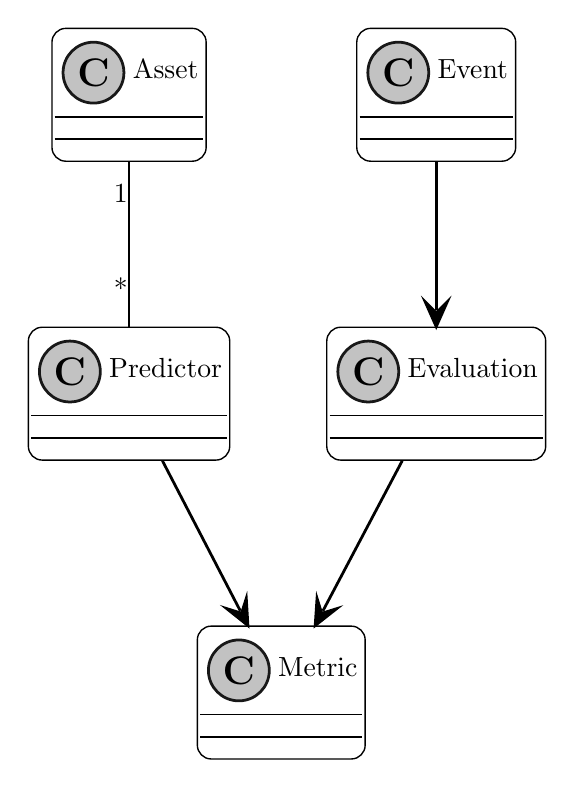
\begin{tikzpicture}[yscale=-1
,pstyle0/.style={color=black,fill=white,line width=0.5pt}
,pstyle1/.style={color=plantucolor0003,fill=plantucolor0002,line width=1.0pt}
,pstyle2/.style={color=black,line width=0.5pt}
,pstyle3/.style={color=black,line width=1.0pt}
,pstyle4/.style={color=black,fill=black,line width=1.0pt}
]
\draw[pstyle0] (15.53pt,12pt) arc (180:270:5pt) -- (20.53pt,7pt) -- (66.24pt,7pt) arc (270:360:5pt) -- (71.24pt,12pt) -- (71.24pt,50pt) arc (0:90:5pt) -- (66.24pt,55pt) -- (20.53pt,55pt) arc (90:180:5pt) -- (15.53pt,50pt) -- cycle;
\draw[pstyle1] (30.53pt,23pt) ellipse (11pt and 11pt);
\node at (30.53pt,23pt)[]{\textbf{\Large C}};
\node at (44.53pt,18pt)[below right,color=black,inner sep=0]{Asset};
\draw[pstyle2] (16.53pt,39pt) -- (70.24pt,39pt);
\draw[pstyle2] (16.53pt,47pt) -- (70.24pt,47pt);
\draw[pstyle0] (125.67pt,12pt) arc (180:270:5pt) -- (130.67pt,7pt) -- (178.09pt,7pt) arc (270:360:5pt) -- (183.09pt,12pt) -- (183.09pt,50pt) arc (0:90:5pt) -- (178.09pt,55pt) -- (130.67pt,55pt) arc (90:180:5pt) -- (125.67pt,50pt) -- cycle;
\draw[pstyle1] (140.67pt,23pt) ellipse (11pt and 11pt);
\node at (140.67pt,23pt)[]{\textbf{\Large C}};
\node at (154.67pt,18pt)[below right,color=black,inner sep=0]{Event};
\draw[pstyle2] (126.67pt,39pt) -- (182.09pt,39pt);
\draw[pstyle2] (126.67pt,47pt) -- (182.09pt,47pt);
\draw[pstyle0] (7pt,120pt) arc (180:270:5pt) -- (12pt,115pt) -- (74.76pt,115pt) arc (270:360:5pt) -- (79.76pt,120pt) -- (79.76pt,158pt) arc (0:90:5pt) -- (74.76pt,163pt) -- (12pt,163pt) arc (90:180:5pt) -- (7pt,158pt) -- cycle;
\draw[pstyle1] (22pt,131pt) ellipse (11pt and 11pt);
\node at (22pt,131pt)[]{\textbf{\Large C}};
\node at (36pt,126pt)[below right,color=black,inner sep=0]{Predictor};
\draw[pstyle2] (8pt,147pt) -- (78.76pt,147pt);
\draw[pstyle2] (8pt,155pt) -- (78.76pt,155pt);
\draw[pstyle0] (68.06pt,228pt) arc (180:270:5pt) -- (73.06pt,223pt) -- (123.7pt,223pt) arc (270:360:5pt) -- (128.7pt,228pt) -- (128.7pt,266pt) arc (0:90:5pt) -- (123.7pt,271pt) -- (73.06pt,271pt) arc (90:180:5pt) -- (68.06pt,266pt) -- cycle;
\draw[pstyle1] (83.06pt,239pt) ellipse (11pt and 11pt);
\node at (83.06pt,239pt)[]{\textbf{\Large C}};
\node at (97.06pt,234pt)[below right,color=black,inner sep=0]{Metric};
\draw[pstyle2] (69.06pt,255pt) -- (127.7pt,255pt);
\draw[pstyle2] (69.06pt,263pt) -- (127.7pt,263pt);
\draw[pstyle0] (114.83pt,120pt) arc (180:270:5pt) -- (119.83pt,115pt) -- (188.93pt,115pt) arc (270:360:5pt) -- (193.93pt,120pt) -- (193.93pt,158pt) arc (0:90:5pt) -- (188.93pt,163pt) -- (119.83pt,163pt) arc (90:180:5pt) -- (114.83pt,158pt) -- cycle;
\draw[pstyle1] (129.83pt,131pt) ellipse (11pt and 11pt);
\node at (129.83pt,131pt)[]{\textbf{\Large C}};
\node at (143.83pt,126pt)[below right,color=black,inner sep=0]{Evaluation};
\draw[pstyle2] (115.83pt,147pt) -- (192.93pt,147pt);
\draw[pstyle2] (115.83pt,155pt) -- (192.93pt,155pt);
\draw[pstyle3] (43.38pt,55.26pt) ..controls (43.38pt,72.94pt) and (43.38pt,97.13pt) .. (43.38pt,114.79pt);
\node at (37.7068pt,63.1236pt)[below right,color=black,inner sep=0]{1};
\node at (37.7081pt,96.9398pt)[below right,color=black,inner sep=0]{*};
\draw[pstyle3] (154.38pt,55.26pt) ..controls (154.38pt,72.94pt) and (154.38pt,91.13pt) .. (154.38pt,108.79pt);
\draw[pstyle4] (154.38pt,114.79pt) -- (158.38pt,105.79pt) -- (154.38pt,109.79pt) -- (150.38pt,105.79pt) -- (154.38pt,114.79pt) -- cycle;
\draw[pstyle3] (55.45pt,163.26pt) ..controls (64.62pt,180.94pt) and (74.405pt,199.8051pt) .. (83.575pt,217.4651pt);
\draw[pstyle4] (86.34pt,222.79pt) -- (85.7425pt,212.9593pt) -- (84.0358pt,218.3526pt) -- (78.6426pt,216.6459pt) -- (86.34pt,222.79pt) -- cycle;
\draw[pstyle3] (142.09pt,163.26pt) ..controls (132.75pt,180.94pt) and (122.7728pt,199.8249pt) .. (113.4428pt,217.4849pt);
\draw[pstyle4] (110.64pt,222.79pt) -- (118.3809pt,216.7008pt) -- (112.9756pt,218.3691pt) -- (111.3074pt,212.9638pt) -- (110.64pt,222.79pt) -- cycle;
\end{tikzpicture}
}
%     % \caption{Class diagram for the Metric abstraction.}
%     \label{fig:irie-classes}
% \end{figure}

\begin{figure}[H]
    \centering
    \resizebox{0.9\linewidth}{!}{% generated by Plantuml 1.2025.4       
\definecolor{plantucolor0000}{RGB}{0,0,0}
\definecolor{plantucolor0001}{RGB}{255,255,255}
\definecolor{plantucolor0002}{RGB}{24,24,24}
\definecolor{plantucolor0003}{RGB}{227,227,227}
\definecolor{plantucolor0004}{RGB}{238,238,238}
\begin{tikzpicture}[yscale=-1
,pstyle0/.style={color=black,line width=1.5pt}
,pstyle1/.style={color=plantucolor0001,line width=0.0pt}
,pstyle2/.style={color=plantucolor0002,line width=0.5pt,dash pattern=on 5.0pt off 5.0pt}
,pstyle3/.style={color=plantucolor0002,fill=plantucolor0003,line width=0.5pt}
,pstyle4/.style={color=plantucolor0002,fill=plantucolor0002,line width=1.0pt}
,pstyle5/.style={color=plantucolor0002,line width=1.0pt}
]
\draw[pstyle0] (112.14pt,140pt) rectangle (400.44pt,247pt);
\draw[pstyle1] (38.45pt,40pt) rectangle (46.45pt,312pt);
\draw[pstyle2] (42pt,40pt) -- (42pt,312pt);
\draw[pstyle1] (172.23pt,40pt) rectangle (180.23pt,312pt);
\draw[pstyle2] (176.14pt,40pt) -- (176.14pt,312pt);
\draw[pstyle1] (278.19pt,40pt) rectangle (286.19pt,312pt);
\draw[pstyle2] (281.975pt,40pt) -- (281.975pt,312pt);
\draw[pstyle1] (391.44pt,40pt) rectangle (399.44pt,312pt);
\draw[pstyle2] (395.285pt,40pt) -- (395.285pt,312pt);
\draw[pstyle1] (439.955pt,40pt) rectangle (447.955pt,312pt);
\draw[pstyle2] (443.595pt,40pt) -- (443.595pt,312pt);
\draw[pstyle3] (5pt,20pt) arc (180:270:5pt) -- (10pt,15pt) -- (74.9pt,15pt) arc (270:360:5pt) -- (79.9pt,20pt) -- (79.9pt,34pt) arc (0:90:5pt) -- (74.9pt,39pt) -- (10pt,39pt) arc (90:180:5pt) -- (5pt,34pt) -- cycle;
\node at (12pt,22pt)[below right,color=black,inner sep=0]{Web Gateway};
\draw[pstyle3] (5pt,316pt) arc (180:270:5pt) -- (10pt,311pt) -- (74.9pt,311pt) arc (270:360:5pt) -- (79.9pt,316pt) -- (79.9pt,330pt) arc (0:90:5pt) -- (74.9pt,335pt) -- (10pt,335pt) arc (90:180:5pt) -- (5pt,330pt) -- cycle;
\node at (12pt,318pt)[below right,color=black,inner sep=0]{Web Gateway};
\draw[pstyle3] (122.14pt,10pt) arc (180:270:5pt) -- (127.14pt,5pt) -- (225.32pt,5pt) arc (270:360:5pt) -- (230.32pt,10pt) -- (230.32pt,34pt) arc (0:90:5pt) -- (225.32pt,39pt) -- (127.14pt,39pt) arc (90:180:5pt) -- (122.14pt,34pt) -- cycle;
\node at (146.31pt,12pt)[below right,color=black,inner sep=0]{Orchestration};
\node at (129.14pt,22pt)[below right,color=black,inner sep=0]{(Evaluation Daemon)};
\draw[pstyle3] (122.14pt,316pt) arc (180:270:5pt) -- (127.14pt,311pt) -- (225.32pt,311pt) arc (270:360:5pt) -- (230.32pt,316pt) -- (230.32pt,340pt) arc (0:90:5pt) -- (225.32pt,345pt) -- (127.14pt,345pt) arc (90:180:5pt) -- (122.14pt,340pt) -- cycle;
\node at (146.31pt,318pt)[below right,color=black,inner sep=0]{Orchestration};
\node at (129.14pt,328pt)[below right,color=black,inner sep=0]{(Evaluation Daemon)};
\draw[pstyle3] (248.975pt,20pt) arc (180:270:5pt) -- (253.975pt,15pt) -- (310.405pt,15pt) arc (270:360:5pt) -- (315.405pt,20pt) -- (315.405pt,34pt) arc (0:90:5pt) -- (310.405pt,39pt) -- (253.975pt,39pt) arc (90:180:5pt) -- (248.975pt,34pt) -- cycle;
\node at (255.975pt,22pt)[below right,color=black,inner sep=0]{Predictor [i]};
\draw[pstyle3] (248.975pt,316pt) arc (180:270:5pt) -- (253.975pt,311pt) -- (310.405pt,311pt) arc (270:360:5pt) -- (315.405pt,316pt) -- (315.405pt,330pt) arc (0:90:5pt) -- (310.405pt,335pt) -- (253.975pt,335pt) arc (90:180:5pt) -- (248.975pt,330pt) -- cycle;
\node at (255.975pt,318pt)[below right,color=black,inner sep=0]{Predictor [i]};
\draw[pstyle3] (371.285pt,10pt) arc (180:270:5pt) -- (376.285pt,5pt) -- (414.595pt,5pt) arc (270:360:5pt) -- (419.595pt,10pt) -- (419.595pt,34pt) arc (0:90:5pt) -- (414.595pt,39pt) -- (376.285pt,39pt) arc (90:180:5pt) -- (371.285pt,34pt) -- cycle;
\node at (378.285pt,12pt)[below right,color=black,inner sep=0]{Domain};
\node at (383.275pt,22pt)[below right,color=black,inner sep=0]{Layer};
\draw[pstyle3] (371.285pt,316pt) arc (180:270:5pt) -- (376.285pt,311pt) -- (414.595pt,311pt) arc (270:360:5pt) -- (419.595pt,316pt) -- (419.595pt,340pt) arc (0:90:5pt) -- (414.595pt,345pt) -- (376.285pt,345pt) arc (90:180:5pt) -- (371.285pt,340pt) -- cycle;
\node at (378.285pt,318pt)[below right,color=black,inner sep=0]{Domain};
\node at (383.275pt,328pt)[below right,color=black,inner sep=0]{Layer};
\draw[pstyle3] (429.595pt,20pt) arc (180:270:5pt) -- (434.595pt,15pt) -- (453.315pt,15pt) arc (270:360:5pt) -- (458.315pt,20pt) -- (458.315pt,34pt) arc (0:90:5pt) -- (453.315pt,39pt) -- (434.595pt,39pt) arc (90:180:5pt) -- (429.595pt,34pt) -- cycle;
\node at (436.595pt,22pt)[below right,color=black,inner sep=0]{DB};
\draw[pstyle3] (429.595pt,316pt) arc (180:270:5pt) -- (434.595pt,311pt) -- (453.315pt,311pt) arc (270:360:5pt) -- (458.315pt,316pt) -- (458.315pt,330pt) arc (0:90:5pt) -- (453.315pt,335pt) -- (434.595pt,335pt) arc (90:180:5pt) -- (429.595pt,330pt) -- cycle;
\node at (436.595pt,318pt)[below right,color=black,inner sep=0]{DB};
\draw[pstyle4] (164.23pt,73pt) -- (174.23pt,77pt) -- (164.23pt,81pt) -- (168.23pt,77pt) -- cycle;
\draw[pstyle5] (42.45pt,77pt) -- (170.23pt,77pt);
\node at (49.45pt,54pt)[below right,color=black,inner sep=0]{POST /events};
\node at (49.45pt,65pt)[below right,color=black,inner sep=0]{(sensor payload)};
\draw[pstyle4] (431.955pt,97pt) -- (441.955pt,101pt) -- (431.955pt,105pt) -- (435.955pt,101pt) -- cycle;
\draw[pstyle5] (176.23pt,101pt) -- (437.955pt,101pt);
\node at (183.23pt,89pt)[below right,color=black,inner sep=0]{insert Event};
\draw[pstyle4] (383.44pt,121pt) -- (393.44pt,125pt) -- (383.44pt,129pt) -- (387.44pt,125pt) -- cycle;
\draw[pstyle5] (176.23pt,125pt) -- (389.44pt,125pt);
\node at (183.23pt,113pt)[below right,color=black,inner sep=0]{query active Predictors};
\draw[color=black,fill=plantucolor0004,line width=1.5pt] (112.14pt,140pt) -- (178.54pt,140pt) -- (178.54pt,142pt) -- (168.54pt,152pt) -- (112.14pt,152pt) -- (112.14pt,140pt);
\draw[pstyle0] (112.14pt,140pt) rectangle (400.44pt,247pt);
\node at (127.14pt,141pt)[below right,color=black,inner sep=0]{\textbf{loop}};
\node at (193.54pt,142pt)[below right,color=black,inner sep=0]{\textbf{[for each Predictor]}};
\draw[pstyle4] (270.19pt,164pt) -- (280.19pt,168pt) -- (270.19pt,172pt) -- (274.19pt,168pt) -- cycle;
\draw[pstyle5] (176.23pt,168pt) -- (276.19pt,168pt);
\node at (183.23pt,156pt)[below right,color=black,inner sep=0]{launch(i, EventID)};
\draw[pstyle5] (282.19pt,192pt) -- (324.19pt,192pt);
\draw[pstyle5] (324.19pt,192pt) -- (324.19pt,205pt);
\draw[pstyle5] (283.19pt,205pt) -- (324.19pt,205pt);
\draw[pstyle4] (293.19pt,201pt) -- (283.19pt,205pt) -- (293.19pt,209pt) -- (289.19pt,205pt) -- cycle;
\node at (289.19pt,180pt)[below right,color=black,inner sep=0]{init→execute→harvest};
\draw[pstyle4] (187.23pt,235pt) -- (177.23pt,239pt) -- (187.23pt,243pt) -- (183.23pt,239pt) -- cycle;
\draw[color=plantucolor0002,line width=1.0pt,dash pattern=on 2.0pt off 2.0pt] (181.23pt,239pt) -- (281.19pt,239pt);
\node at (193.23pt,217pt)[below right,color=black,inner sep=0]{Metric set};
\node at (193.23pt,227pt)[below right,color=black,inner sep=0]{+ provenance};
\draw[pstyle4] (431.955pt,266pt) -- (441.955pt,270pt) -- (431.955pt,274pt) -- (435.955pt,270pt) -- cycle;
\draw[pstyle5] (176.23pt,270pt) -- (437.955pt,270pt);
\node at (183.23pt,258pt)[below right,color=black,inner sep=0]{insert Evaluation + Metrics};
\draw[pstyle4] (53.45pt,290pt) -- (43.45pt,294pt) -- (53.45pt,298pt) -- (49.45pt,294pt) -- cycle;
\draw[pstyle5] (47.45pt,294pt) -- (175.23pt,294pt);
\node at (59.45pt,282pt)[below right,color=black,inner sep=0]{notify(evaluation\_ready)};
\end{tikzpicture}
}
    \caption{Sequence diagram illustrating the process of evaluating an event.}
    \label{fig:irie-sequences}
\end{figure}
The \gls{event} and \gls{evaluation} abstractions provide a general framework for capturing and processing data from the physical system, enabling the digital twin to reflect the state of the physical system accurately and in real time.
In the context of bridge health monitoring, this generally corresponds to any situation that could place the health of a structure in jeopardy
and for which an \gls{evaluation} is desired, but more generally, may also be used to represent any relaying of data from the physical structure to the digital twin. 
The processing of an \gls{event} generally culminates in the creation of an \gls{evaluation}, which is expected to be of immediate interest to the user or the decision-maker.

\subsubsection{Event Abstraction}

The \gls{event} abstraction represents any occurrence that results in data being relayed from the physical system to the digital twin. An \gls{event} could be a routine data collection, a triggered sensor reading due to a significant change in the physical system, or any other situation that necessitates the transfer of data for processing and analysis.
%
This abstraction is designed to be broad and flexible, accommodating a wide range of scenarios and data types.
It allows the digital twin to respond to changes in the physical system promptly and accurately, regardless of the nature or cause of the \gls{event}.

\begin{Note}

An example of how SGMD \cite{mccallen2025open-access} can be leveraged to advance structural resilience research is through its integration with existing structural health monitoring platforms.

As a practical application of these advancements, integrating SGMD with \BRACE{} can significantly enhance structural health monitoring efforts. 

Data driven methods are currently limited by data sparsity, particularly for structures without instrumentation. 
Integrating SGMD with \BRACE{} addresses this limitation by enabling preemptive analysis through simulated ground motions. This integration allows for predictive modeling for structures lacking sensor data, improving the ability to forecast structural responses during future seismic events. Additionally, SGMD data can inform real-time assessments by providing baseline models against which real-time sensor data can be compared, enhancing the accuracy of structural health evaluations. This integration extends the benefits of \BRACE{} to a broader range of infrastructure within the transportation network, contributing to more comprehensive community resilience.
\end{Note}

\subsubsection{Evaluation Abstraction}

The \gls{evaluation} abstraction represents the process of analyzing the data received from an \gls{event}. This involves invoking the appropriate \glspl{predictor}, processing the data, and generating metrics that provide insights into the state and performance of the physical system.
%
The \gls{evaluation} abstraction is designed to be adaptable and scalable, capable of handling a wide range of analysis methods and data volumes. It ensures that the digital twin can provide meaningful and actionable insights, regardless of the complexity or scale of the data.
